در ابتدا state و تابع heuristic را برای مسئله تعریف می‌کنیم.
\begin{enumerate}
    \item :state هر وزیر در یک ستون از 8 ستون می‌باشد.
    \item (state) function :heuristic تعداد وزرایی که همدگیر را تهدید می‌کنند.
    \item در هر گام می‌توانیم یک وزیر را در ستونش جابجا کنیم.
\end{enumerate}


فضای این مسئله شامل 17 میلیون حالت مختلف می‌شود و در 14درصد اوقات به یک جواب مسئله دست می‌یابیم.
در این روش، در حالاتی که یافتن جواب موفقیت‌آمیز بوده است به طور میانگین 4 تغییر state رخ می‌دهد و در حالاتی که الگوریتم نتوانسته است همسایه‌ای بهتر پیدا کند، 3 تغییر state رخ می‌دهد.


شکل زیر نمونه‌ای از یک حالتی است که نمی‌توان آن را بهبود داد.
\begin{figure}[H]
    \centering
    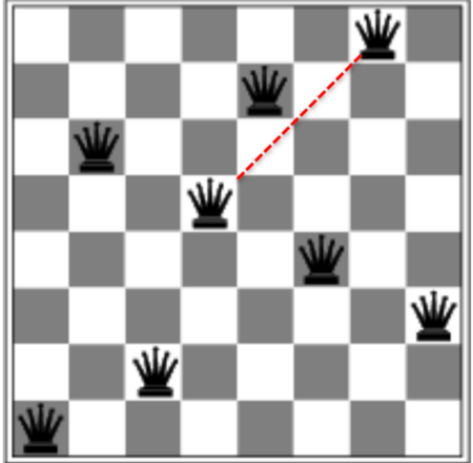
\includegraphics[width=0.4\textwidth]{source/bummer.png}
    \label{fig:bummer}
\end{figure}

برای بهبود درصد موفقیت برای حالاتی مثل شکل بالا که نمی‌توانیم حالاتی بهتر بیابیم، اجازه دهیم تا اگر حالتی وجود داشت که مقدار  h آن با مقدار state  کنونی برابری می‌کرد انتخاب شود.
همچنین برای جلوگیری از وارد حلقه شدن انتخاب state ها می‌‌توانیم یک حد بالا برای تعداد sideway های ممکن تعیین کنیم.
با فرض آنکه حد بالای sideways ها را برابر 100 در نظر بگیریم داریم:

\begin{itemize}
    \item در 94درصد اوقات الگوریتم به یک جواب برای مسئله دست پیدا می‌کند.
    \item در حالات موفق به طور میانگین 21 گام و در حالات ناموفق به طور میانگین 64 گام انجام می‌شود.
\end{itemize}

در روش hill-climbing چالش‌هایی مانند مورد ذکر شده وجود دارد.
تصویر زیر نمونه‌هایی از این چالش‌ها می‌باشند.

\begin{figure}[H]
    \minipage{\textwidth}
    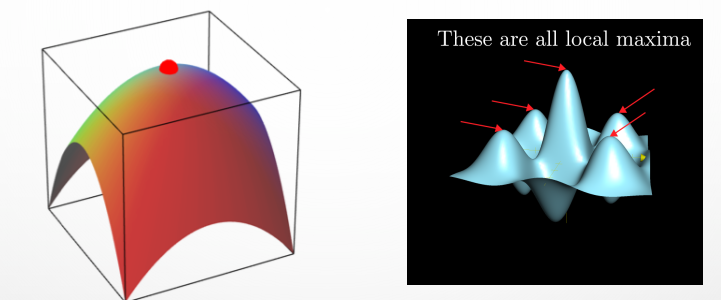
\includegraphics[width=\linewidth]{source/local-maxima.png}
    \caption{local-maxima}
    \label{fig:local-maxima}
    \endminipage\hfill
    \minipage{0.4\textwidth}
    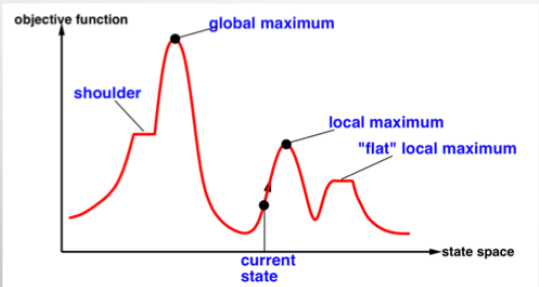
\includegraphics[width=\linewidth]{source/plateus.png}
    \caption{plateus}
    \label{fig:plateus}
    \endminipage\hfill
    \minipage{0.4\textwidth}
    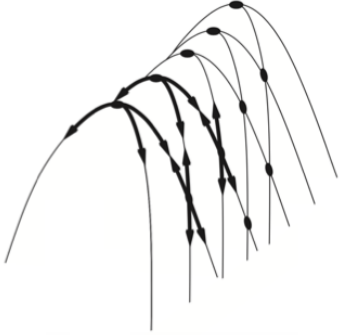
\includegraphics[width=\linewidth]{source/diagonal-ridges.png}
    \caption{diagonal-ridges}
    \label{fig:diagonal-ridges}
    \endminipage\hfill
\end{figure}

